\documentclass[11pt]{article}
\usepackage[margin=1in]{geometry}
\usepackage{mathptmx}
\usepackage{amsmath,amssymb}
\usepackage{graphicx}
\usepackage{booktabs}
\usepackage{multirow}
\usepackage{xcolor}
\usepackage[hidelinks]{hyperref}
\usepackage{caption}
\captionsetup{font=small,labelfont=bf}
\newcommand{\pending}[1]{\textcolor{orange!80!black}{[\textbf{PENDING:} #1]}}

\title{\textbf{Penny-Wise, Cache-Foolish:}\\ When Token-Optimal MCP Tool Retrieval Isn't Cost-Optimal\\[4pt]
\large\normalfont\textcolor{orange!80!black}{[Preprint v1.0 --- 2026-09-23 --- co-authorship unconfirmed, see footnote]}}
\author{Anoshor B.\ Paul\thanks{Corresponding author.}\quad Chirag Pradhan\thanks{\textcolor{orange!80!black}{Authorship unconfirmed at this revision: listed at the corresponding author's request, pending each co-author's review of the manuscript, agreement to be named, and a CRediT statement of their actual contribution. Remove or confirm before circulation.}}\quad Krishn Maloo\footnotemark[2]\\[4pt] Independent Researchers\\ \texttt{anoshorpaul@gmail.com}}
\date{}

\begin{document}
\maketitle

\begin{abstract}
Agents built on the Model Context Protocol (MCP) increasingly face catalogs of hundreds of tools, and a growing literature proposes retrieving only the relevant tool schemas to shrink the prompt. These methods report their efficiency as \emph{raw token reduction}. Commercial LLM APIs, however, bill cached prompt prefixes at roughly one tenth of the uncached price and may charge a premium to write them, so the token count a method minimizes is not the quantity a deployment pays for. We analyze this gap with a closed-form cost model of tool exposure under prefix caching and a trace-driven counterfactual replay of 95 real LiveMCPBench trajectories (525 MCP tools, 119k schema tokens) under four verified provider pricing regimes. For a single short task, retrieval is both token- and cost-optimal, costing 0.09$\times$ as much as loading every tool with caching. As sessions grow, however, the ranking inverts. In ten-task sessions over a 100-tool catalog, per-step retrieval sends 42\% fewer tokens yet costs 1.60$\times$ more (cluster-valid 95\% CI 1.45--1.74 over disjoint sessions), and is more expensive in every session we replay. Our pre-registered hypothesis that retrieval-in-prefix costs more than static caching for sessions of $\geq$20 calls and $\leq$150 tools holds under all three tested regimes (1.25--1.37$\times$). We derive a break-even rule (retrieval pays only when the omitted catalog exceeds $\frac{W-R}{2R}\,\bar h\,(m-1)$ tokens) that predicts the replay's break-even catalog size within 7.8\% mean error under Anthropic/OpenAI pricing. Two design choices matter more than the retrieval algorithm. Placing retrieved schemas \emph{after} the conversation history is the cheapest strategy in every ten-task configuration of the replay grid, though the one cell we could bill puts it level with per-request retrieval. Non-deterministic schema serialization alone inflates static-caching cost 1.7--4.8$\times$. A live billing check on \texttt{gpt-5-nano} (1,151 requests) puts the replay within 17.4\% of billed cost and shows that it \emph{understates} the real cost of retrieval, so the reported crossover is conservative. Tool-selection accuracy meanwhile falls from 71\% to 41\% as the exposed catalog grows from 16 to 128 tools, so neither exposing everything nor re-selecting per turn is free; pricing those errors shrinks the inversion region without eliminating it.
\end{abstract}

\noindent\textbf{Keywords:} Model Context Protocol, tool retrieval, prompt caching, LLM agents, inference cost, context engineering

%==================================================================
\section{Introduction}
The Model Context Protocol (MCP) standardizes how LLM applications discover and invoke external tools~\cite{mcp}. Its success has created a scaling problem: an agent connected to a handful of MCP servers can see hundreds of tools, and their JSON schemas are re-sent to the model on every call. The prevailing response is \emph{tool retrieval}: select the few tools relevant to the current request and expose only their schemas. RAG-MCP reports a prompt-token reduction of over 50\%~\cite{ragmcp}, MCP-Zero a 98\% reduction on APIBank~\cite{mcpzero}, vector-based discovery 99.6\%~\cite{semdisc}, and Tool Attention a 95\% reduction in tool tokens per turn~\cite{toolattention}.

These numbers share a unit, the raw input token, that is no longer what commercial APIs bill. Anthropic, OpenAI and Google all cache prompt \emph{prefixes}. Tokens that match an earlier request are billed at about 0.1$\times$ the base input price, while writing a new prefix costs 1.0--2.0$\times$ depending on provider and time-to-live~\cite{anth_cache,oai_cache,gemini_price}. Tool definitions sit at the very start of that prefix. Changing which tools are exposed therefore invalidates not only the tool block but \emph{everything after it}, including a conversation history that may be much larger than the tools themselves~\cite{anth_cache}. A method that minimizes tokens by changing the tool set can, in principle, raise the bill.

Whether it does in practice has not been measured. Lumer et al.\ evaluate prompt caching on long-horizon agents and advise against dynamic function calling, but test no retrieval method and give no cost model~\cite{dontbreak}. Tool Attention places retrieved schemas late in the prompt to protect the cache, but its cost figures are projections rather than billed measurements~\cite{toolattention}. TokenPilot relocates tool definitions downstream and measures real cache hits on one model, without comparing MCP retrieval strategies~\cite{tokenpilot}. Provider-native tool search (\texttt{defer\_loading}) injects discovered tools at the end of the context expressly to preserve the cache~\cite{anth_toolsearch,oai_toolsearch}, but has not been independently compared with the academic retrievers.

This paper asks: \emph{under current prefix-cache pricing, when is token-optimal MCP tool retrieval also cost-optimal, and when is it not?} The scope is deliberately narrow: one single-agent benchmark, API-billed models, and cost measured at the billing interface rather than inside a serving stack. We make five contributions:
\begin{enumerate}
\item A closed-form cost model of tool exposure under prefix caching, with a break-even rule for when retrieval pays off (Section~\ref{sec:model}).
\item A trace-driven counterfactual replay that bills nine exposure strategies over 95 real LiveMCPBench trajectories, 525 real MCP tool schemas and four verified pricing regimes, at zero API cost (Section~\ref{sec:method}).
\item Evidence that the token and cost rankings agree for single short tasks but \emph{invert} in multi-task sessions, confirming a pre-registered hypothesis, and that the break-even rule predicts where the inversion begins (Section~\ref{sec:results}).
\item Practical guidance: cache-aware \emph{placement} of retrieved schemas matters more for cost than the choice of retriever (Section~\ref{sec:discussion}).
\item Evidence that a mechanical defect, non-deterministic serialization of tool definitions, can cost more than every strategy choice in this paper combined, and is free to fix (Section~\ref{sec:serial}).
\end{enumerate}

%==================================================================
\section{Background and Related Work}
\label{sec:related}
\paragraph{MCP and tool exposure.} An MCP client aggregates tools from one or more servers and presents them to the model, usually as function definitions in the request's \texttt{tools} field. Benchmarks such as LiveMCPBench (95 tasks, 70 servers, 527 tools)~\cite{livemcpbench}, MCP-Bench~\cite{mcpbench}, MCP-Universe~\cite{mcpuniverse} and MCP-AgentBench~\cite{mcpagentbench} evaluate agents on real servers; they report success and, at most, raw token usage. Hasan et al.\ show that most MCP tool descriptions contain quality defects that affect selection~\cite{smelly}, which bears on how large each schema is.

\paragraph{Tool retrieval.} RAG-MCP retrieves relevant tool descriptions from an external index before calling the model~\cite{ragmcp}. MCP-Zero lets the agent actively request tools as it works~\cite{mcpzero}. Semantic tool discovery embeds tools and retrieves the top-$k$ per query~\cite{semdisc}. Tool Attention keeps compact summaries of all tools in the prompt and loads full schemas only for gated tools, placing them just before the latest user message~\cite{toolattention}. Code-execution designs expose tools as a programmatic API instead of function definitions~\cite{cemcp}; we leave them to future work.

\paragraph{Prompt caching.} All three major providers cache prompt prefixes. Anthropic bills cache writes at 1.25$\times$ (5-minute TTL) or 2$\times$ (1-hour TTL) and reads at 0.1$\times$. Its prefix hierarchy runs \emph{tools $\rightarrow$ system $\rightarrow$ messages}, and a change at any level invalidates all later levels~\cite{anth_cache}. OpenAI caches automatically. On GPT-5.6 and later, writes cost 1.25$\times$ and reads 0.1$\times$, while earlier models have no write premium; any change to tool names, descriptions, schemas or ordering prevents reuse~\cite{oai_cache}. Gemini's implicit cache bills cached tokens at 0.1$\times$ (e.g., \$0.075 vs.\ \$0.75 per million on Gemini 3.8 Flash) with a 4,096-token minimum~\cite{gemini_price}. Lumer et al.\ measure 41--80\% cost savings from caching across providers~\cite{dontbreak}. TokenPilot reconciles context compression with cache alignment~\cite{tokenpilot}. ReCache makes KV blocks composition-invariant for self-hosted serving~\cite{recache}, which does not help API users. A public gateway issue documents tool-schema property order changing between syncs in 44\% of consecutive request pairs, silently breaking the cache~\cite{bifrost}.

\paragraph{Gap.} No prior work gives a cost model for tool-exposure strategies under prefix caching, compares the retrieval families on the same real traces with cache-aware billing, or tests whether the token ranking reported by retrieval papers survives caching.

%==================================================================
\section{A Cost Model of Tool Exposure}
\label{sec:model}
\paragraph{Billing.} Normalize the uncached input price to 1. Suppose a call's prompt has $x$ tokens in total, of which the first $c$ match a prefix already in the cache. Its input costs $R\,c + W\,(x-c)$, where $R$ is the read multiplier and $W$ the write multiplier. Output tokens cost $O$ each. Cached tokens count only when the shared prefix reaches the provider's minimum length.

\paragraph{Prompt layout.} At call $t$ the prompt is a tool block $B_t$, a system prompt $S$, and an append-only history $H_t$. Strategies differ only in what $B_t$ contains and where retrieved schemas sit (Table~\ref{tab:strategies}). Let $C$ be the tokens of the full catalog, $b$ the tokens of a retrieved subset, $\bar h$ the mean tokens appended per call, $T$ the number of calls and $m$ the number of user requests (tasks) in the session.

\paragraph{Break-even for per-request retrieval.} A static cached catalog pays for $C$ once at the write price and then at the read price on each call. Retrieval that changes the tool set at each new request saves $(C-b)$ tokens on every call, worth about $(C-b)\,[\,W + R(T-1)\,]$ over the session. But each change invalidates the history behind it: at the $j$-th request, the history of roughly $(j-1)\,\bar h\,T/m$ tokens is written at $W$ instead of read at $R$. Summing over the $m-1$ switches gives an extra cost of $(W-R)\,\bar h\,T\,(m-1)/2$. Retrieval is cheaper if and only if
\begin{equation}
C - b \;>\; \frac{(W-R)\,\bar h\,T\,(m-1)}{2\,(R\,T + W - R)} \;\;\xrightarrow{\;T\gg 1\;}\;\; \frac{W-R}{2R}\,\bar h\,(m-1).
\label{eq:breakeven}
\end{equation}
Under Anthropic's 5-minute pricing or OpenAI GPT-5.6+ ($W{=}1.25$, $R{=}0.1$) the constant $\frac{W-R}{2R}$ is 5.75; without a write premium ($W{=}1$) it is 4.5. In words, \emph{retrieval pays only if the tools you leave out are worth more tokens than about six turns' worth of history growth, per re-retrieval.} The saving grows with the catalog, but the penalty grows with the history, and history grows with session length.

\paragraph{Per-step retrieval.} If the tool set changes on a fraction $q$ of calls rather than once per request, the same argument gives a threshold of about $\frac{W-R}{2R}\,q\,\bar h\,T$, which grows with $T$ itself.

\paragraph{Placement.} Equation~\ref{eq:breakeven} assumes retrieved schemas sit in the prefix. If instead they are placed after the history (tail placement) or appended when discovered (append-only), a change in the tool set leaves the history's cache intact, and the cache-break term disappears. The price is that tail schemas are re-sent uncached on every call, and appended schemas accumulate.

\begin{table}[t]
\centering\small
\caption{Tool-exposure strategies replayed. ``Prefix'' means the retrieved schemas occupy the tool block at the start of the prompt.}
\label{tab:strategies}
\begin{tabular}{@{}lll@{}}
\toprule
ID & Strategy & Represents \\
\midrule
S0 & All schemas in prefix, caching disabled & Lower bound \\
S1 & All schemas in prefix, cached & Naive production default \\
S1u & S1 with tool JSON re-serialized non-deterministically ($p{=}0.44$/call) & Gateway bug~\cite{bifrost} \\
S2 & Retrieved schemas in prefix, re-retrieved per step & MCP-Zero-style active discovery~\cite{mcpzero} \\
S2r & Retrieved schemas in prefix, retrieved per request & RAG-MCP-style~\cite{ragmcp} \\
S2u & Prefix holds the union of everything retrieved so far & ``Sticky'' fix \\
S3 & Summaries of all tools in prefix; retrieved schemas after history & Tool Attention layout~\cite{toolattention} \\
S4 & Two meta-tools; discovery results appended to history & Recorded agent; Anthropic tool search~\cite{anth_toolsearch} \\
S5 & Names+descriptions in prefix; schemas appended on discovery & OpenAI tool search~\cite{oai_toolsearch} \\
\bottomrule
\end{tabular}
\end{table}

%==================================================================
\section{Methodology}
\label{sec:method}
\paragraph{Data.} We use all 95 trajectories released with LiveMCPBench~\cite{livemcpbench}. They were produced by a Claude Sonnet 4 agent that discovers tools through a \texttt{route} meta-tool backed by Qwen3-Embedding retrieval and invokes them through an \texttt{execute-tool} meta-tool. Each trajectory records every assistant message, tool call and tool result, and carries a judge-assigned success label (0.74 success rate under the Claude Sonnet 4 judge). We tokenize all messages and the benchmark's 525 parseable tool schemas with the \texttt{o200k\_base} tokenizer. The catalog totals 119,374 schema tokens (mean 227, median 137, maximum 2,044 per tool). Trajectories average 9.5 LLM calls (6.5 excluding pure discovery calls), and each non-discovery call appends $\bar h = 949$ tokens on average. All 222 distinct tools returned by retrieval match catalog entries.

\paragraph{Counterfactual replay.} Cost depends only on the \emph{shape} of the token flow (which segments appear, in what order, at each call) and on provider billing rules. For each trajectory and strategy we reconstruct the ordered segments of every prompt the strategy would send, holding the agent's actions fixed. Strategies without a discovery tool (S0--S3) drop the route-only calls and their results, since those calls would not exist.
\begin{itemize}
\item For S2, the retrieved set at each call is the most recent route result.
\item For S2r, it is the union of the task's route results, fixed for the duration of the request (an optimistic retriever).
\item For S2u, it is the union of everything retrieved so far in the session.
\end{itemize}
Each call is billed by the rule of Section~\ref{sec:model}, with the cached prefix computed as the longest segment-exact prefix shared with an earlier prompt in the session. Because history is append-only, the most recent earlier prompt with the same tool block always gives the longest match, so replay is linear in session length. Output is billed at $O{=}5$.

\paragraph{Sessions and catalogs.} Real assistants serve several requests per conversation. We form 95 sessions of $m \in \{1,2,3,5,10\}$ tasks by chaining trajectories in a fixed seeded order, so that each task starts exactly one session. A new request appends the user's question to the history and triggers per-request retrieval. The catalog for a session of size $N \in \{25,50,100,200,525\}$ always contains every tool the session retrieves or executes, filled to $N$ with a seeded random sample of the remaining tools.

\paragraph{Pricing regimes.} All four were verified against provider documentation on 2026-09-19:
\begin{itemize}
\item P1: $W{=}1.25$, $R{=}0.1$, minimum 1,024 tokens (Anthropic 5-minute TTL; OpenAI GPT-5.6+)~\cite{anth_cache,oai_cache}.
\item P2: $W{=}1$, $R{=}0.1$, minimum 1,024 (OpenAI GPT-5.5 and earlier)~\cite{oai_cache}.
\item P3: $W{=}2$, $R{=}0.1$, minimum 1,024 (Anthropic 1-hour TTL)~\cite{anth_cache}.
\item P4: $W{=}1$, $R{=}0.1$, minimum 4,096 (Gemini implicit caching)~\cite{gemini_price}.
\end{itemize}

\paragraph{Statistics and hypotheses.} We report per-session cost ratios against S1 with 95\% percentile-bootstrap confidence intervals (4,000 resamples, paired by session). Before any replay we registered four hypotheses in the project's Phase-1 scoping record:
\begin{itemize}
\item \textbf{H1:} for $N \leq 150$ and $T \geq 20$ calls, retrieval-in-prefix costs more than static caching under at least two of three regimes.
\item \textbf{H2:} the analytical model predicts billed cost within 20\% MAPE.
\item \textbf{H3:} cache-aware placement is on the cost--accuracy Pareto frontier for $N \geq 100$.
\item \textbf{H4:} static exposure loses selection accuracy as $N$ grows.
\end{itemize}

\paragraph{Accuracy proxy.} Replay cannot measure how exposure changes agent behavior. As a zero-cost proxy we compute \emph{availability}: the share of executed tools that were inside each retrieval-in-prefix strategy's tool set at the moment of execution. A tool outside the set could not have been called.

\paragraph{Live validation.} A harness replays each strategy's exact prompt sequence against \texttt{gpt-5-nano} (\$0.05 per million uncached and \$0.005 per million cached input tokens~\cite{oai_price}) with a 64-token output allowance. It reads the billed \texttt{cached\_tokens} to test H2 against real billing, measures tool-selection accuracy with $N \in \{16,32,64,128\}$ candidate tools (H4), and probes the reported 128-tool request limit~\cite{oai_limit}. The whole run is guarded by a hard \$1.50 cap; Section~\ref{sec:live} reports the outcome.

%==================================================================
\section{Results}
\label{sec:results}
\subsection{Single tasks: token-optimal is cost-optimal}
Table~\ref{tab:single} shows the replay for one task per session with the full 525-tool catalog under P1. Every retrieval variant costs about a tenth of static caching (S2r 0.09$\times$, 95\% CI 0.08--0.10), and the token and cost rankings largely agree. Measured churn is low: once discovery calls are removed, the retrieved set changes between consecutive calls in only 7\% of cases on average (median 0\%). The agent retrieves early and then executes, so a prefix-resident tool set is rarely invalidated within a task. Results under P2--P4 are qualitatively identical. P4's 4,096-token minimum lowers cache hits for the small retrieved prefixes (S2 hit rate 22\% vs.\ 46\%), but S2 still costs only 0.11$\times$.

\begin{table}[t]
\centering\small
\caption{Single-task sessions, $N{=}525$, pricing P1. Cost is the mean per-task ratio to S1 with 95\% bootstrap CI.}
\label{tab:single}
\begin{tabular}{@{}lrrrr@{}}
\toprule
Strategy & Raw input tokens/task & Cost vs.\ S1 & 95\% CI & Cache hit \\
\midrule
S0 static, no cache & 807,818 & 3.10 & [2.85, 3.37] & 0\% \\
S1 static, cached & 807,818 & 1.00 & --- & 75\% \\
S1u static, unstable JSON & 807,818 & 2.29 & [2.10, 2.48] & 41\% \\
S2 RAG-prefix, per step & 31,495 & 0.09 & [0.08, 0.10] & 46\% \\
S2r RAG-prefix, per request & 41,377 & 0.09 & [0.08, 0.10] & 55\% \\
S2u RAG-prefix, sticky union & 38,950 & 0.10 & [0.08, 0.11] & 50\% \\
S3 summaries + tail schemas & 103,634 & 0.18 & [0.17, 0.19] & 68\% \\
S4 discovery, append-only & 54,354 & 0.10 & [0.09, 0.11] & 60\% \\
S5 name+desc + append & 312,138 & 0.34 & [0.33, 0.35] & 82\% \\
\bottomrule
\end{tabular}
\end{table}

\subsection{Sessions: the ranking inverts}
Figure~\ref{fig:heatmap} maps the cost of per-request retrieval (S2r) relative to static caching across session length and catalog size. Retrieval's advantage shrinks with every additional request in the session and grows with catalog size. With three tasks per session it already loses at $N{=}25$ (1.12$\times$). With ten tasks it loses up to $N{=}100$ (1.31$\times$) and breaks even at $N{=}200$ (1.00$\times$). Only the full 525-tool catalog keeps retrieval ahead at ten tasks (0.56$\times$).

\begin{figure}[t]
\centering
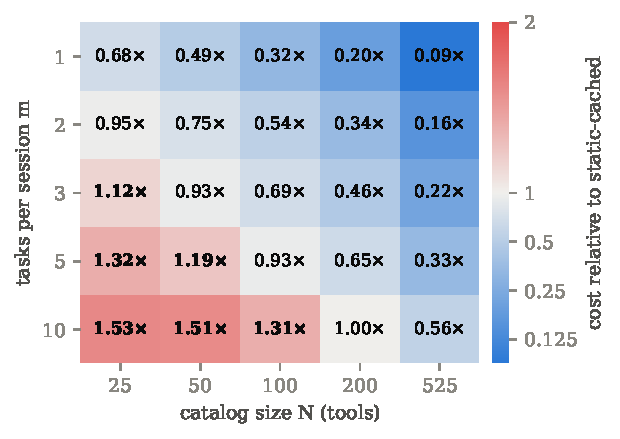
\includegraphics[width=0.62\linewidth]{figs/fig1_heatmap_S2r_P1.pdf}
\caption{Cost of per-request retrieval-in-prefix (S2r) relative to static caching (S1), pricing P1. Blue: retrieval cheaper; red (bold): static caching cheaper. Each cell averages 95 sessions.}
\label{fig:heatmap}
\end{figure}

Table~\ref{tab:h1} tests the pre-registered H1 over every session with at least 20 LLM calls and $N \in \{25, 50, 100, 150\}$. Per-step retrieval (S2) costs 1.25--1.37$\times$ static caching under all three regimes, and every confidence interval excludes 1. Per-request retrieval (S2r) costs 1.07--1.15$\times$. \textbf{H1 is supported} under three of three regimes, where two were required.

\begin{table}[t]
\centering\small
\caption{H1: sessions with $\geq$20 LLM calls and $N{\in}\{25,50,100,150\}$ ($n{=}880$ session--catalog pairs per row).}
\label{tab:h1}
\begin{tabular}{@{}llrrr@{}}
\toprule
Regime & Strategy & Mean cost vs.\ S1 & 95\% CI & Sessions costlier than S1 \\
\midrule
\multirow{2}{*}{P1 ($W{=}1.25$)} & S2 per step & 1.37 & [1.34, 1.40] & 78\% \\
 & S2r per request & 1.15 & [1.13, 1.17] & 68\% \\
\multirow{2}{*}{P2 ($W{=}1.00$)} & S2 per step & 1.25 & [1.22, 1.27] & 73\% \\
 & S2r per request & 1.07 & [1.05, 1.09] & 60\% \\
\multirow{2}{*}{P4 (Gemini)} & S2 per step & 1.28 & [1.25, 1.30] & 76\% \\
 & S2r per request & 1.10 & [1.08, 1.12] & 64\% \\
\bottomrule
\end{tabular}
\end{table}

\subsection{Fewer tokens, higher bill}
Figure~\ref{fig:inversion} plots raw input tokens against cost for $N{=}100$. For a single task the two axes agree: strategies that send fewer tokens cost less. For ten-task sessions they disagree. Per-step retrieval (S2) sends 2.08M tokens per session against static caching's 3.57M (42\% fewer), yet costs 1.60$\times$ as much (95\% CI 1.56--1.65) and is more expensive than S1 in all 95 sessions. The sticky-union ``fix'' (S2u) is the worst retrieval variant at 1.82$\times$: every newly retrieved tool changes the prefix, and the prefix only grows.

\begin{figure}[t]
\centering
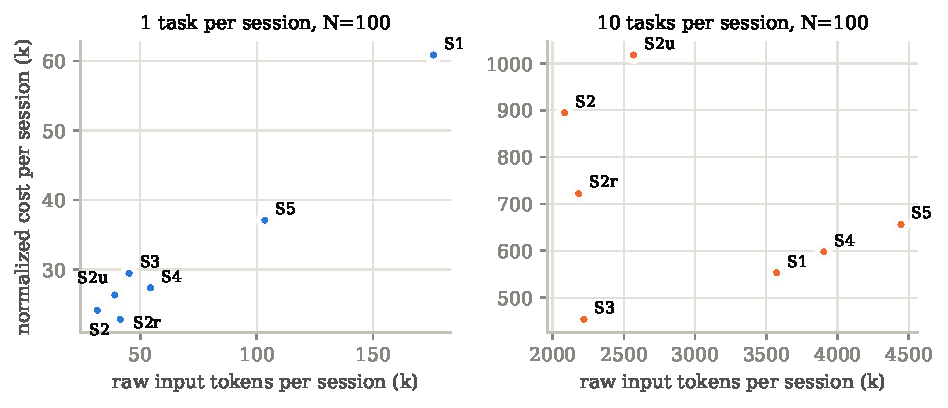
\includegraphics[width=\linewidth]{figs/fig3_inversion_P1_N100.pdf}
\caption{Raw input tokens (the metric retrieval papers report) versus normalized cost, $N{=}100$, P1. Left: single task. Right: ten-task sessions, where the lowest-token strategies (S2, S2r, S2u) are among the most expensive.}
\label{fig:inversion}
\end{figure}

\subsection{Placement beats retrieval}
Figure~\ref{fig:bars} compares all strategies at $N{=}100$. Tail placement (S3) is the most robust design. In ten-task sessions it is the cheapest strategy at every catalog size under all three regimes of the replay grid (Section~\ref{sec:reconcile} qualifies this against billed data), e.g., 0.94$\times$, 0.82$\times$ and 0.40$\times$ static caching at $N{=}25$, 100 and 525 under P1. Its worst cell across the whole grid is 1.02$\times$ under P1, 0.99$\times$ under P2 and 1.13$\times$ under P4, where Gemini's 4,096-token minimum hurts it in short sessions over small catalogs. Append-only discovery (S4, the recorded agent's own design) is next, with a worst cell of 1.24--1.27$\times$, and it beats static caching in ten-task sessions only for larger catalogs. Per-request retrieval remains the best choice for single tasks, but the placement-aware designs trail it by 0.02--0.17 of S1's cost.

\begin{figure}[t]
\centering
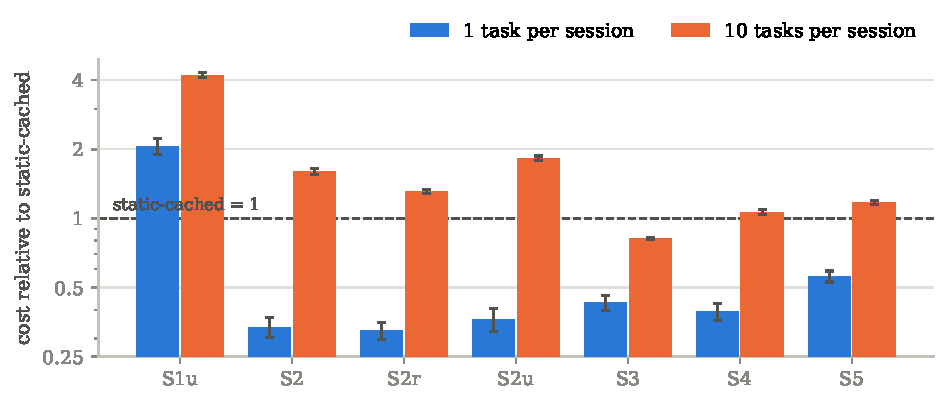
\includegraphics[width=\linewidth]{figs/fig2_strategies_P1_N100.pdf}
\caption{Cost relative to static caching (dashed line) at $N{=}100$, P1, for one-task (blue) and ten-task (orange) sessions. Error bars: 95\% bootstrap CI. S1u = unstable serialization; S2/S2r/S2u = retrieval in prefix; S3 = summaries + tail schemas; S4/S5 = append-only discovery.}
\label{fig:bars}
\end{figure}

\subsection{Serialization stability can dominate every other choice}
\label{sec:serial}
The 44\% churn rate we use as input comes from a single production gateway report~\cite{bifrost} and should be read as an illustrative rate, not an ecosystem constant; the mechanism, not the rate, is the finding. Randomly re-serializing the tool JSON on 44\% of calls raises static-caching cost 1.7--4.8$\times$ across the P1 grid (Figure~\ref{fig:serial}). The penalty grows with session length and catalog size. In ten-task sessions with 100 tools this single defect costs 4.20$\times$ (95\% CI 4.10--4.31), more than any choice between exposure strategies.

\begin{figure}[t]
\centering
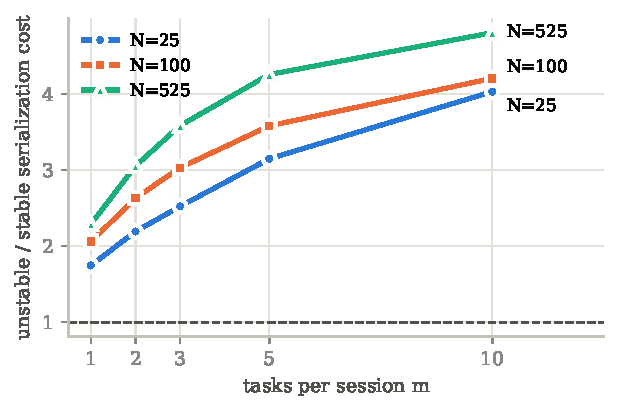
\includegraphics[width=0.55\linewidth]{figs/fig4_serialization_P1.pdf}
\caption{Cost of static caching with non-deterministic schema serialization ($p{=}0.44$ per call) relative to stable serialization, P1.}
\label{fig:serial}
\end{figure}

\subsection{The break-even rule predicts the crossover}
Table~\ref{tab:breakeven} compares the break-even catalog size predicted by Equation~\ref{eq:breakeven} with the size at which the replay's mean S2r/S1 ratio crosses 1 (log-interpolated on a 17-point grid). The prediction uses the measured $\bar h{=}949$, 6.5 calls per task and a 1,680-token retrieved set. Under P1 and P2 the rule is within 4--11\% in every cell (mean absolute percentage error 7.8\%). Under P4 it underestimates short sessions (by 51\% at $m{=}2$), because Gemini's 4,096-token minimum prevents small prefixes from caching at all, which Equation~\ref{eq:breakeven} does not model; the error falls to 7\% by $m{=}10$. The overall MAPE across the 12 cells is 14.4\%. A first version of the rule, which omitted the one-time write term and averaged per-task ratios, overestimated break-even by about 40\%; we report the corrected derivation.

\begin{table}[t]
\centering\small
\caption{Break-even catalog size $N^*$ (tools): Equation~\ref{eq:breakeven} versus replay.}
\label{tab:breakeven}
\begin{tabular}{@{}lrrrrrrrr@{}}
\toprule
 & \multicolumn{2}{c}{$m{=}2$} & \multicolumn{2}{c}{$m{=}3$} & \multicolumn{2}{c}{$m{=}5$} & \multicolumn{2}{c}{$m{=}10$} \\
\cmidrule(lr){2-3}\cmidrule(lr){4-5}\cmidrule(lr){6-7}\cmidrule(lr){8-9}
Regime & pred. & replay & pred. & replay & pred. & replay & pred. & replay \\
\midrule
P1 & 19 & 20 & 36 & 40 & 76 & 84 & 189 & 198 \\
P2 & 17 & 18 & 32 & 35 & 64 & 71 & 154 & 161 \\
P4 & 17 & 34 & 32 & 47 & 64 & 80 & 154 & 165 \\
\bottomrule
\end{tabular}
\end{table}

\subsection{Accuracy proxy and sensitivity}
Per-step retrieval would have hidden the tool the agent actually executed in 35\% of calls (availability 64.8\%, 342 of 528 executions). Per-request (99.2\%) and sticky (98.5\%) sets almost never miss, although S2r achieves this with an optimistic retriever that knows the task's full tool needs. For per-step retrieval, cost and accuracy therefore point the same way: it is both the most cache-hostile and the most likely to hide the needed tool. We also randomly expired the cache on 10\% or 30\% of calls, as a proxy for TTL expiry during slow tool execution. This narrows the advantage of caching (S0 falls from 3.49$\times$ to 1.74$\times$ of S1 at 30\%) but leaves the single-task ordering of strategies unchanged. Varying the output-to-input price ratio from $O{=}5$ to $O{=}0$ or $O{=}8$ does not change which strategy is cheapest in any tested cell. At $m{=}10$, $N{=}100$, per-step retrieval costs 1.73$\times$ static caching at $O{=}0$ and 1.54$\times$ at $O{=}8$.

\subsection{Live billing validation}
\label{sec:live}
We replayed ten three-task sessions ($N{=}100$) for four strategies against \texttt{gpt-5-nano}: 1,151 requests, 15.0M billed input tokens (13.2M served from cache), \$0.19. All live experiments in this paper, including the selection test and one discarded batch, cost \$0.58.

\paragraph{Tool-count limit (E0).} Requests carrying 129 and all 525 tool definitions were both \emph{accepted}. The 128-tool ceiling reported by users of other OpenAI endpoints does not apply to the Responses API on this model, so catalog size is limited by context and cost rather than by a hard cap.

\paragraph{Predicted vs.\ billed (H2).} Table~\ref{tab:live} compares the replay's prediction with the provider's own \texttt{cached\_tokens}. The mean absolute percentage error on per-sequence input cost is 17.4\%, inside the 20\% we pre-registered, so \textbf{H2 is supported}. Two systematic deviations matter. First, billed cache hit rates run 3--7 points below prediction, because OpenAI caches in 128-token increments above a 1,024-token minimum and its cache is best-effort, while the replay assumes an exact-prefix, always-available cache. Second, and more importantly, the \emph{advantage} of every non-static strategy is smaller in billing than in replay: S2r costs 0.70$\times$ static caching rather than the predicted 0.53$\times$, and S4 costs 1.08$\times$ rather than 0.66$\times$. The replay therefore \emph{overstates} what retrieval and discovery save, which means the cost crossover of Section~\ref{sec:results} arrives \emph{earlier} in real billing than our replay places it. Our central claim is conservative under this bias.

\begin{table}[t]
\centering\small
\caption{Live validation on \texttt{gpt-5-nano} (10 sessions $\times$ 3 tasks, $N{=}100$, 1,151 requests). Cost ratios are per session against S1.}
\label{tab:live}
\begin{tabular}{@{}lrrrr@{}}
\toprule
 & \multicolumn{2}{c}{Cache hit rate} & \multicolumn{2}{c}{Cost vs.\ S1} \\
\cmidrule(lr){2-3}\cmidrule(lr){4-5}
Strategy & billed & predicted & billed & predicted \\
\midrule
S1 static, cached & 89\% & 94\% & 1.00 & 1.00 \\
S2r RAG-prefix, per request & 76\% & 83\% & 0.70 & 0.53 \\
S3 summaries + tail schemas & 81\% & 85\% & 0.72 & 0.51 \\
S4 discovery, append-only & 88\% & 94\% & 1.08 & 0.66 \\
\bottomrule
\end{tabular}
\end{table}

\paragraph{Practitioner pitfalls found while measuring.} Two mechanical issues cost us a full measurement run and are worth reporting. (i) Several real MCP servers publish JSON-Schema draft-04 artefacts (a boolean \texttt{exclusiveMinimum}) that the API rejects outright; a client that forwards MCP schemas unmodified will fail on them. (ii) When \texttt{max\_output\_tokens} is small enough that the model exhausts it during reasoning, the response returns \texttt{incomplete} with \emph{all usage fields zero}, so a naive measurement harness silently records no tokens. Anyone measuring cache behavior on reasoning models should assert that usage is non-zero.

\paragraph{Selection accuracy (H4).} For each of 93 tasks we asked the model to choose the tool the recorded agent actually executed, among $N$ candidates drawn from the same catalog. Accuracy falls monotonically as the catalog grows: 71.0\% at $N{=}16$ (95\% Wilson CI 61.1--79.2), 61.3\% at 32, 54.3\% at 64 and 40.9\% at 128 (31.4--51.0). On the 93 tasks answered at both sizes, moving from 16 to 128 candidates flips 30 tasks from correct to incorrect and only 2 in the other direction (McNemar $\chi^2 = 22.8$, $p < 0.0001$). \textbf{H4 is supported}: exposing a large catalog costs selection accuracy, which is the counterweight to the cost advantage static caching gains in long sessions.

\paragraph{A reproducibility caveat.} An earlier collection of the same 372 items, run in several resumed batches over four days, produced an anomalous 8.6\% at $N{=}16$ in which the model selected the first listed tool in 93 of 93 cases, while agreeing with the reported run at $N \geq 32$ (58.1\%, 53.8\%, 35.5\%). We could not reproduce that degenerate behavior in fresh probes of the same items and report the single-batch run instead, with the anomaly recorded here. Model aliases can change under a long-running experiment; measurements of this kind should be collected in one batch and the exact model snapshot recorded.

\subsection{Robustness of the central claim}
\label{sec:robust}
Three assumptions carry most of the weight in the results above. We test each.

\paragraph{Sessions overlap, so the intervals above are too narrow.} Each task begins one session and reappears in the $m-1$ sessions that follow it, so the paired bootstrap treats correlated sessions as independent. We therefore rebuild the grid from \emph{disjoint} sessions, in which no task is reused (9 sessions at $m{=}10$, 31 at $m{=}3$). The point estimates barely move and the intervals widen as expected: per-step retrieval at $m{=}10$, $N{=}100$ is 1.60$\times$ with a cluster-valid interval of [1.45, 1.74] (against [1.56, 1.65] from overlapping sessions), and at $N{=}25$ it is 1.84$\times$ [1.71, 1.99]. Tail placement is 0.82$\times$ [0.81, 0.84]. Every interval that matters still excludes 1, so the inversion survives valid inference; we treat the disjoint intervals as the load-bearing ones.

\paragraph{The per-request retriever was an oracle.} S2r's tool set is the union of what the recorded router actually returned, which no deployed retriever knows in advance. Replacing it with a real BM25 retriever over tool names, descriptions and parameter names, queried with the user's request, leaves cost essentially unchanged (1.30$\times$ vs.\ 1.31$\times$ at $m{=}10$, $N{=}100$, since set size is what drives cost) but collapses quality: the BM25 top-5 contains the tool the agent actually executed in only \textbf{18.3\%} of executions, against 64.8\% for the trace's embedding router and 99.2\% for the oracle. The retrieval cost estimates in this paper are therefore \emph{generous} to retrieval: they price a retriever far better than a simple lexical one.

\paragraph{Holding agent behavior fixed favours static exposure.} Section~\ref{sec:live} shows selection accuracy falling with catalog size, so a static-exposure agent should make more wrong calls and pay for them. We add that cost: interpolating the measured accuracy to each strategy's visible schema count and charging one extra call per wrong selection. The effect runs \emph{against} our headline rather than for it, because static exposure is the strategy penalised most and it is the denominator. At $m{=}10$, $N{=}100$, per-step retrieval moves from 1.62$\times$ to 1.38$\times$; at $N{=}200$ it moves from 1.23$\times$ to 0.97$\times$. The inversion therefore holds at moderate catalogs, but its boundary moves inward once selection errors are priced, and at $N{=}200$ it disappears. We report this as a limit on the claim, not as support for it.

\subsection{What the billed data do and do not confirm}
\label{sec:reconcile}
The replay ranks tail placement (S3) ahead of per-request retrieval (S2r) everywhere, but the single cell we could bill puts them level: 0.72$\times$ and 0.70$\times$ at $m{=}3$, $N{=}100$ (Table~\ref{tab:live}), where the replay predicted 0.51$\times$ and 0.53$\times$. Two conclusions follow. First, the \emph{ordering} of the cheap strategies is not established by billing; our placement recommendation rests on the replay grid and on the mechanism, not on a measured win. Second, the replay's error is not uniform across strategies: append-only discovery was predicted at 0.66$\times$ and billed at 1.08$\times$, a 64\% relative error on precisely the design both major providers ship. Readers should treat the replay as reliable for the direction and magnitude of the \emph{static-versus-retrieval} comparison, which the billing reproduces, and as unreliable for fine distinctions among the cache-friendly designs.

%==================================================================
\section{Discussion}
\label{sec:discussion}
\paragraph{Guidance for MCP client and gateway builders.}
\begin{enumerate}
\item \textbf{Serialize tool definitions deterministically.} Canonical key order and stable tool order cost nothing, and non-determinism erased most of caching's benefit in our replay.
\item \textbf{Do not put a changing tool set at the top of the prompt in a long conversation.} If tools must change, place their schemas after the history (S3) or append them (S4, provider tool search).
\item \textbf{Do the break-even arithmetic.} Per-request retrieval into the prefix pays only if the omitted catalog exceeds about $\frac{W-R}{2R}\bar h (m{-}1)$ tokens, roughly 5.75 turns' worth of history growth per re-retrieval under 1.25/0.1 pricing.
\item \textbf{Growing the tool set monotonically is not a fix.} Every addition is a prefix change.
\item \textbf{For short, single-request agents, retrieval is fine.} The token-reduction results in the literature hold there.
\item \textbf{Loading everything is cheap, not free.} Selection accuracy fell from 71\% to 41\% as the visible catalog grew from 16 to 128 tools (Section~\ref{sec:live}). Static caching's cost advantage in long sessions is paid for in accuracy, which is exactly why placement-aware designs are attractive: they keep the model's visible tool set small \emph{and} keep the prefix stable.
\end{enumerate}

\paragraph{A decision procedure.} Measure $\bar h$ (tokens your turns add) and $m$ (requests per conversation); compute the threshold $\frac{W-R}{2R}\,\bar h\,(m-1)$; compare it with the token size of the catalog you would omit. Above the threshold, retrieve; below it, load everything once and keep the prefix stable; in either case put schemas that change \emph{after} the history. For the workload measured here ($\bar h = 949$, six calls per request), the threshold is roughly 5.5k tokens per additional request under 1.25/0.1 pricing, i.e.\ about 24 average tools.

\paragraph{What this is worth in money.} At the verified \texttt{gpt-5-nano} rate (\$0.05/M input, \$0.005/M cached), 1,000 ten-task sessions over a 100-tool catalog cost \$27.65 with static caching, \$44.73 with per-step retrieval and \$22.68 with tail placement: a \$17 penalty per thousand sessions for the token-minimizing choice, and \$5 of savings for the placement-aware one. Scale linearly for frontier-model rates.

\paragraph{Two stakeholders beyond client authors.} MCP \emph{server} authors set the catalog term directly: the median tool in our catalog costs 137 tokens and the largest costs 2,044, so trimming the tail moves the break-even more cheaply than any client-side change. \emph{Providers} could remove the serialization hazard outright by canonicalizing tool definitions before hashing the prefix, and could make the trade-off visible by reporting tool-block tokens separately in usage.

\paragraph{Implications for research.} Tool-retrieval papers should report cost under at least one cache-aware billing model, over multi-request sessions, alongside raw tokens. Raw-token reductions measured on single queries overstate savings for conversational deployments and can reverse their sign. Benchmarks that already release full trajectories, as LiveMCPBench does, make this analysis free.

\paragraph{Implications for the protocol.} MCP's \texttt{tools/list\_changed} notification lets a server change the tool list mid-session. Our results suggest that clients should treat such changes as append events rather than rebuilding the tool block, and that the specification could recommend canonical serialization of tool definitions.

%==================================================================
\section{Threats to Validity}
\paragraph{Internal.} Replay holds agent behavior fixed across strategies, whereas in reality the tools the model sees change what it does, including how many calls it makes. We partly address this with the availability proxy and the pending live accuracy test, but cost differences below roughly 10\% should not be over-interpreted. Caching is modeled as deterministic; real caches are best-effort and quantized to 128-token increments, which we do not model. Section~\ref{sec:live} measures the resulting bias: it favours the non-static strategies, so our crossover estimates are conservative.
\paragraph{Construct.} We use one tokenizer (\texttt{o200k\_base}) as a proxy for all providers and an output-to-input price ratio of 5. The conclusions do not depend on that ratio (Section~\ref{sec:results}). List prices differ from negotiated prices, so we report ratios and publish token counts by type for repricing.
\paragraph{External.} The strategy \emph{ordering} among cache-friendly designs is not confirmed by billing (Section~\ref{sec:reconcile}), and our retrieval costs assume a retriever much stronger than BM25 (Section~\ref{sec:robust}). All trajectories come from one agent (Claude Sonnet 4 with an embedding router) on one benchmark. Multi-task sessions are synthesized by chaining independent tasks, which lacks the cross-task context reuse of real conversations. S2r's retrieved sets come from the agent's own discovery calls and are optimistic.
\paragraph{Conclusion validity.} H1, H2 and H4 are supported, H1 under cluster-valid intervals from disjoint sessions. H1's window ($N \leq 150$, $T \geq 20$) describes a regime, not the ecosystem, and long sessions are synthesized rather than observed. H3 is supported directly on the cost side; on the accuracy side it rests on an inference (S3 and S4 expose about five schemas at a time, close to our $N{=}16$ condition, whereas static exposure at $N{\geq}100$ sits near our 128-candidate condition), not on a measurement of those strategies end to end. The break-even rule's agreement is with our replay, not yet with billed cost.

%==================================================================
\section{Conclusion}
Token-optimal MCP tool retrieval is cost-optimal for single short tasks and cost-foolish for long multi-request sessions over moderate catalogs, where re-selecting tools invalidates an ever-larger cached history. A simple rule predicts the crossover, and pricing selection errors moves it inward without removing it. Two engineering choices outweigh the choice of retriever: where retrieved schemas are placed, and whether tool definitions serialize deterministically. We recommend that future tool-retrieval work report cache-aware cost over sessions, not raw tokens over queries.

%==================================================================
\section*{Declarations}
\paragraph{Data availability.} Code (trace extraction, replay, break-even analysis, figures and live-validation harness) and derived data is available at \url{https://github.com/Anoshor/penny-wise-cache-foolish} (MIT license). LiveMCPBench is available under the Apache-2.0 license~\cite{livemcpbench}.
\paragraph{Ethics.} This study uses only publicly released benchmark trajectories and involves no human participants or personal data.
\paragraph{Author contributions (CRediT).} A.\,B.\,Paul: Conceptualization, Methodology, Software, Formal analysis, Investigation, Writing -- original draft, Writing -- review \& editing. \pending{C.\ Pradhan and K.\ Maloo: contributions to be stated by each co-author, who must also confirm they have read and approved the manuscript. Authorship is not established until then.}
\paragraph{Competing interests.} The author works in industry on agentic AI systems. No employer data, systems or internal findings were used, and the work was conducted independently. \pending{author to confirm wording}
\paragraph{Funding.} None.
\paragraph{Use of AI tools.} An AI assistant (Claude, Anthropic) was used for literature search, code development, analysis and drafting under the author's direction. The author reviewed all content and takes full responsibility for it. Pricing figures from Anthropic, OpenAI and Google documentation were retrieved on 2026-09-19.

%==================================================================
\begin{thebibliography}{99}\small
\bibitem{mcp} Anthropic, ``Introducing the Model Context Protocol,'' Nov.\ 25, 2024. [Online]. Available: \url{https://www.anthropic.com/news/model-context-protocol}
\bibitem{ragmcp} T.~Gan and Q.~Sun, ``RAG-MCP: Mitigating prompt bloat in LLM tool selection via retrieval-augmented generation,'' arXiv:2505.03275, 2025.
\bibitem{mcpzero} X.~Fei, X.~Zheng, and H.~Feng, ``MCP-Zero: Active tool discovery for autonomous LLM agents,'' arXiv:2506.01056, 2025.
\bibitem{semdisc} S.~Mudunuri, J.~Wan, A.~Qin, and S.~Manoharan, ``Semantic tool discovery for large language models: A vector-based approach to MCP tool selection,'' arXiv:2603.20313, 2026.
\bibitem{toolattention} A.~Sadani and D.~Kumar, ``Tool attention is all you need: Dynamic tool gating and lazy schema loading for eliminating the MCP/tools tax in scalable agentic workflows,'' arXiv:2604.21816, 2026.
\bibitem{dontbreak} E.~Lumer, F.~Nizar, A.~Jangiti, K.~Frank, A.~Gulati, M.~Phadate, and V.~K.~Subbiah, ``Don't break the cache: An evaluation of prompt caching for long-horizon agentic tasks,'' arXiv:2601.06007, 2026.
\bibitem{tokenpilot} B.~Xu \emph{et al.}, ``TokenPilot: Cache-efficient context management for LLM agents,'' arXiv:2606.17016, 2026.
\bibitem{recache} Y.~Fang, S.~Wei, H.~Hu, and X.~Shen, ``ReCache: Efficient KV cache reuse and compression for tool-augmented LLM agents,'' arXiv:2608.19662, 2026.
\bibitem{livemcpbench} G.~Mo, W.~Zhong, J.~Chen, Q.~Yuan, X.~Chen, Y.~Lu, H.~Lin, B.~He, X.~Han, and L.~Sun, ``LiveMCPBench: Can agents navigate an ocean of MCP tools?'' arXiv:2508.01780, 2025.
\bibitem{mcpbench} Z.~Wang \emph{et al.}, ``MCP-Bench: Benchmarking tool-using LLM agents with complex real-world tasks via MCP servers,'' arXiv:2508.20453, 2025.
\bibitem{mcpuniverse} Z.~Luo \emph{et al.}, ``MCP-Universe: Benchmarking large language models with real-world Model Context Protocol servers,'' arXiv:2508.14704, 2025.
\bibitem{mcpagentbench} Z.~Guo, B.~Xu, C.~Zhu, W.~Hong, X.~Wang, and Z.~Mao, ``MCP-AgentBench: Evaluating real-world language agent performance with MCP-mediated tools,'' arXiv:2509.09734, 2025.
\bibitem{smelly} M.~M.~Hasan, H.~Li, G.~K.~Rajbahadur, B.~Adams, and A.~E.~Hassan, ``Model Context Protocol (MCP) tool descriptions are smelly! Towards improving AI agent efficiency with augmented MCP tool descriptions,'' arXiv:2602.14878, 2026.
\bibitem{cemcp} Y.~Felendler, P.~A.~Gandhi, I.~Habler, Y.~Elovici, and A.~Shabtai, ``From tool orchestration to code execution: A study of MCP design choices,'' arXiv:2602.15945, 2026.
\bibitem{anth_cache} Anthropic, ``Prompt caching,'' Claude Platform Docs. Accessed: Sep.\ 19, 2026. [Online]. Available: \url{https://platform.claude.com/docs/en/build-with-claude/prompt-caching}
\bibitem{anth_toolsearch} Anthropic, ``Tool search tool,'' Claude Platform Docs. Accessed: Sep.\ 19, 2026. [Online]. Available: \url{https://platform.claude.com/docs/en/agents-and-tools/tool-use/tool-search-tool}
\bibitem{oai_cache} OpenAI, ``Prompt caching,'' OpenAI API Docs. Accessed: Sep.\ 19, 2026. [Online]. Available: \url{https://developers.openai.com/api/docs/guides/prompt-caching}
\bibitem{oai_toolsearch} OpenAI, ``Tool search,'' OpenAI API Docs. Accessed: Sep.\ 19, 2026. [Online]. Available: \url{https://developers.openai.com/api/docs/guides/tools-tool-search}
\bibitem{oai_price} OpenAI, ``Pricing,'' OpenAI API Docs. Accessed: Sep.\ 19, 2026. [Online]. Available: \url{https://developers.openai.com/api/docs/pricing}
\bibitem{gemini_price} Google, ``Gemini Developer API pricing.'' Accessed: Sep.\ 19, 2026. [Online]. Available: \url{https://ai.google.dev/gemini-api/docs/pricing}
\bibitem{bifrost} maximhq/bifrost, ``MCP tool schema property order changes between tool syncs, breaking prompt caching,'' GitHub issue \#7169. [Online]. Available: \url{https://github.com/maximhq/bifrost/issues/7169}
\bibitem{oai_limit} code-yeongyu/oh-my-openagent, ``Too many tools registered (141) exceeds OpenAI API limit of 128,'' GitHub issue \#2848. [Online]. Available: \url{https://github.com/code-yeongyu/oh-my-openagent/issues/2848}
\end{thebibliography}
\end{document}
